% =============================================================================
% Lecture 08: CNN Architectures
% ECON 8310: Business Forecasting
% University of Nebraska at Omaha
% =============================================================================

\documentclass[aspectratio=169, 11pt]{beamer}

\input{header}

% ---- Lecture metadata --------------------------------------------------------
\title[CNN Architectures]{CNN Architectures}
\subtitle{ECON 8310: Business Forecasting --- Lecture 8}
\author{Department of Economics}
\institute{University of Nebraska at Omaha}

% =============================================================================
\begin{document}
% =============================================================================

\begin{frame}
  \titlepage
\end{frame}

% ---- Outline ----------------------------------------------------------------
\begin{frame}{Lecture Outline}
  \tableofcontents
\end{frame}

% =============================================================================
\section{Convolution: The Core Idea}
% =============================================================================

\sectionslide{Convolution: The Core Idea}{%
  Look at a small window, and look for the same thing everywhere.
  Two ideas, and they are the whole architecture.}

% --- Slide: Why convolution (1 of 2: the cost) --------------------------------
\begin{frame}{Why Convolution? A Dense Layer Wastes Its Weights}
  A $224 \times 224$ image has 50{,}176 pixels. One hidden layer of 1{,}000 neurons on top of it
  needs \textbf{50 million weights} --- for one layer. Lecture 7's whole network had 22{,}657.

  \vspace{0.3cm}
  And the waste is worse than the cost. That layer has no idea that \textbf{neighboring pixels
  are related} and distant ones usually are not. And it \textbf{cannot reuse what it learns}: a
  pattern learned in the top-left corner is stored separately from the same pattern in the
  bottom-right.
\end{frame}

% --- Slide: Why convolution (2 of 2: the two ideas) ----------------------------
\begin{frame}{Why Convolution? Two Ideas}
  \begin{center}
    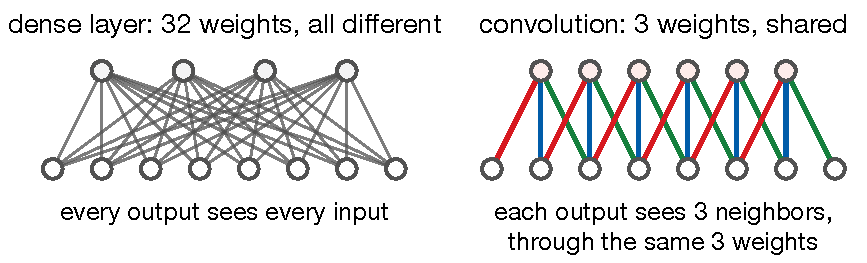
\includegraphics[height=3.0cm]{../Figures/Lecture08/dense_vs_conv.pdf}
  \end{center}
  \begin{keybox}
    \textbf{Local connectivity:} each neuron sees only a small \textbf{receptive field}.
    \textbf{Weight sharing:} the same filter is applied at every position. Far fewer parameters,
    and a pattern learned anywhere is recognized everywhere.
  \end{keybox}
  A reader does not memorize the letter ``A'' separately for every spot on the page. They learn
  it once and apply it everywhere. A filter does exactly that.
\end{frame}

% --- Slide: How convolution works --------------------------------------------
\begin{frame}{How a Convolutional Layer Works}
  For a sequence, a 1D convolution slides a filter of length $K$ along the series and takes a dot
  product at each position:
  \[
    (f * g)[t] = \sum_{k=0}^{K-1} f[k] \cdot g[t - k]
  \]
  \vspace{-0.25cm}
  \begin{center}
    {\small
    \begin{tabular}{p{2.3cm}p{10.1cm}}
      \toprule
      \textbf{Kernel size} & Filter length $K$. Larger means a wider receptive field --- more
      context per output, and more parameters. \\[2pt]
      \textbf{Stride} & How far the filter moves between positions. Stride 2 halves the output
      length. \\[2pt]
      \textbf{Padding} & Zeros at the edges. \texttt{padding='same'} keeps output length equal to
      input length. \\[2pt]
      \textbf{Filters} & How many different patterns to learn. This becomes the number of output
      channels. \\
      \bottomrule
    \end{tabular}
    }
  \end{center}

  Each filter learns one \textbf{local pattern} --- an edge, a spike, a seasonal dip. Its output
  is a \textbf{feature map} whose high values mark where that pattern was found.
\end{frame}

% --- Slide: convolution, worked ----------------------------------------------
\begin{frame}{Convolution, Step by Step}
  A length-10 series and a width-3 filter $[1, 5, 1]$. Slide the filter along and take a dot
  product at each position.
  \begin{center}
    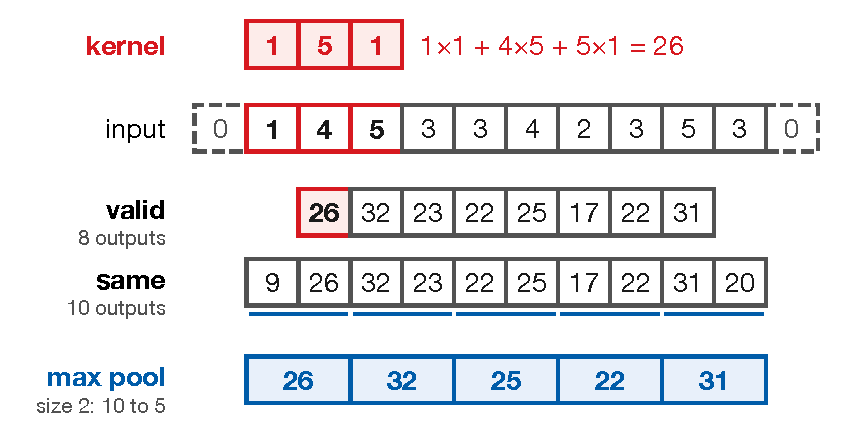
\includegraphics[height=4.9cm]{../Figures/Lecture08/conv1d_step_by_step.pdf}
  \end{center}
  \vspace{-0.2cm}
  {\small \textbf{Valid} keeps only full overlaps: $10 - 3 + 1 = 8$ outputs. \textbf{Same} pads
  a zero at each end and keeps all 10. Max pooling then keeps the larger of each pair.}
\end{frame}

% --- Slide: a filter on a photograph -------------------------------------------
\begin{frame}{What a Filter Sees}
  The same operation in two dimensions: a $3\times3$ filter slides over every pixel of a
  photograph. Two hand-set filters find two different kinds of structure.
  \begin{center}
    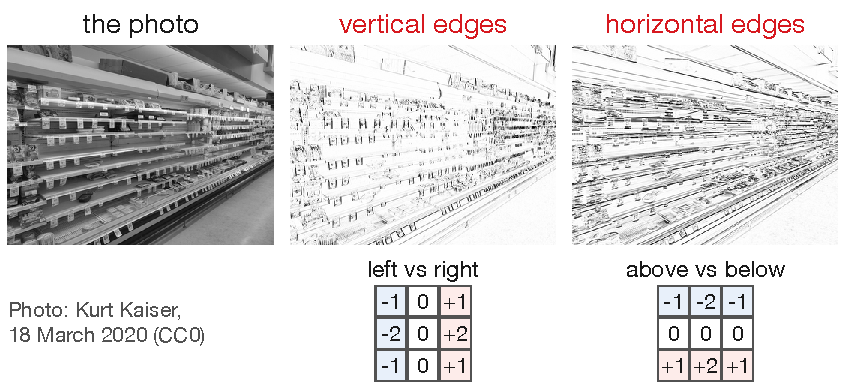
\includegraphics[height=5.3cm]{../Figures/Lecture08/filter_sees.pdf}
  \end{center}
  \vspace{-0.25cm}
  \muted{\small 18 March 2020: shelves emptied by a shock no forecast saw coming --- more in Week 16.}
\end{frame}

% =============================================================================
\section{Pooling and Dropout}
% =============================================================================

\sectionslide{Pooling and Dropout}{%
  Pooling shrinks the feature map and buys robustness ---
  at a price that matters more for forecasting than for images.}

% --- Slide: Pooling ----------------------------------------------------------
\begin{frame}{Pooling: Downsampling Feature Maps}
  \textbf{Pooling} summarizes each small region of a feature map with one number: max pooling
  keeps the largest, average pooling the mean.
  \begin{center}
    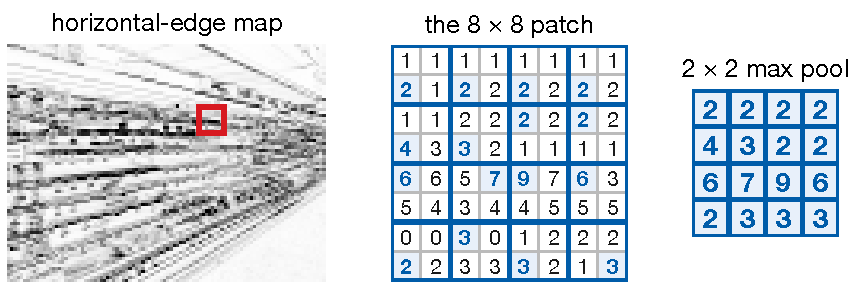
\includegraphics[height=3.0cm]{../Figures/Lecture08/pooling.pdf}
  \end{center}
  \vspace{-0.3cm}
  It buys \textbf{fewer parameters downstream} and \textbf{translation invariance}: shift the
  input slightly and the pooled output barely changes. The shelf edge survives.

  \begin{warningbox}
    \textbf{A feature for images, a problem for forecasting.} A demand spike that moved three
    weeks later is what you are predicting, not noise. Pooling discards \emph{where} a pattern
    occurred --- we measure the cost later in this lecture.
  \end{warningbox}
\end{frame}

% =============================================================================
\section{CNN Architecture Evolution}
% =============================================================================

\sectionslide{CNN Architecture Evolution}{%
  Thirty years of architectures, and three ideas that survived.}

% --- Slide: LeNet to VGG -----------------------------------------------------
\begin{frame}{LeNet to VGG: Depth and Small Filters}
  \textbf{LeNet-5} \parencite{LeCun1998} set the template in 1998: convolution and pooling
  layers, then dense layers. It read handwritten digits on bank checks.

  \vspace{0.15cm}
  \textbf{VGG} \parencite{Simonyan2015} scaled it up in 2014 with one simplification: \emph{only}
  $3\times3$ filters, stacked deep. Two stacked $3\times3$ layers see what one $5\times5$ sees,
  with fewer parameters and an extra nonlinearity.

  \begin{keybox}
    \textbf{The lesson that carried:} depth built from small filters beats width built from large
    ones --- which is why modern architectures are deep and narrow.
  \end{keybox}

  \vspace{0.1cm}
  VGG's cost: 138 million parameters, mostly in the final dense layers.
\end{frame}

% --- Slide: Inception and ResNet ---------------------------------------------
\begin{frame}{Inception and ResNet: Depth That Trains}
  \textbf{Inception} \parencite{Szegedy2015} runs $1\times1$, $3\times3$ and $5\times5$
  convolutions \emph{in parallel} and lets the network choose the scale; $1\times1$
  convolutions keep the cost down.

  \vspace{0.15cm}
  \textbf{ResNet} \parencite{He2016} fixed a different problem: past some depth, deeper networks
  got \emph{worse} --- not from overfitting, but because gradients faded on the way back. The fix
  is a \textbf{residual} or skip connection:
  \begin{center}
    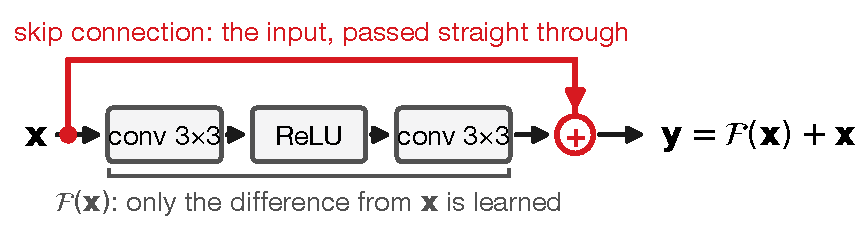
\includegraphics[height=2.4cm]{../Figures/Lecture08/residual_block.pdf}
  \end{center}
  \vspace{-0.3cm}
  The $+\,\mathbf{x}$ gives the gradient a direct path backward. It made 100-layer networks
  trainable, and it is in nearly every deep architecture since --- including Lecture 9's.
\end{frame}

% --- Slide: what a trained network learned --------------------------------------
\begin{frame}{What a Trained CNN Learns}
  ResNet-18, trained on 1.2 million labeled images. Nobody designed its first layer --- these
  are the 64 filters it arrived at, and what four of them find in the same photograph.
  \begin{center}
    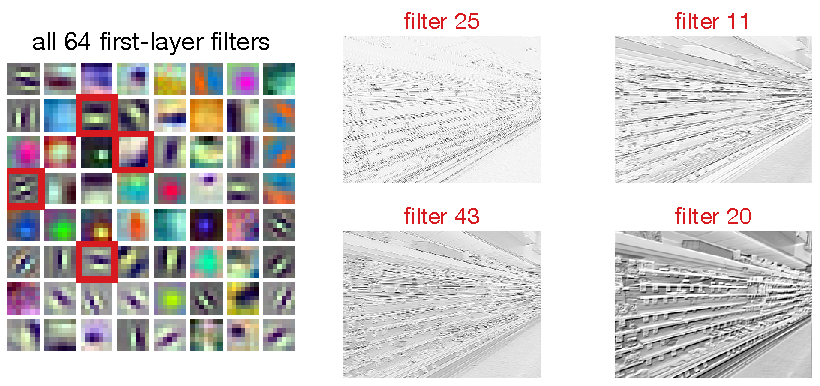
\includegraphics[height=4.9cm]{../Figures/Lecture08/learned_filters.pdf}
  \end{center}
  \vspace{-0.25cm}
  {\small Many look like the edge filters we set by hand; the rest detect color. \textbf{Learned,
  not engineered} --- the same promise a 1D CNN makes for a time series.}
\end{frame}

% --- Slide: what the image architectures taught -------------------------------
\begin{frame}{What Carries Over to Time Series}
  These architectures were built for images, on problems that look nothing like weekly demand
  forecasting. Three of their ideas transfer anyway.

  \vspace{0.1cm}
  \begin{center}
    {\small
    \begin{tabular}{p{3.6cm}p{8.8cm}}
      \toprule
      \textbf{Small stacked filters} & A width-3 filter twice sees six weeks of context with far
      fewer weights than one width-6 filter. \\[3pt]
      \textbf{Skip connections} & Same fix for the same problem --- gradients that fade through
      depth. \\[3pt]
      \textbf{Learned features} & You stop hand-engineering lag windows and let filters find the
      local shapes that matter. \\
      \bottomrule
    \end{tabular}
    }
  \end{center}

  \vspace{0.1cm}
  \textbf{One idea does not transfer, and it is the one we flagged:} pooling for translation
  invariance. An image classifier should not care where the cat is. A forecaster usually should
  care where the spike was.
\end{frame}

% =============================================================================
\section{1D CNNs for Time Series}
% =============================================================================

\sectionslide{1D CNNs for Time Series}{%
  The same machinery, one dimension, and an honest measurement.}

% --- Slide: why 1D CNN -------------------------------------------------------
\begin{frame}{Why Use a 1D CNN for Forecasting?}
  A 1D CNN takes a \textbf{window} of the recent past --- 26 weeks of units, SNAP days, events
  and price --- and predicts the next week. You stop choosing lags: the filters learn which local
  shapes matter. It is far cheaper than a dense network (weight sharing again), and the same
  filters serve \emph{every} store-category at once.
  \begin{center}
    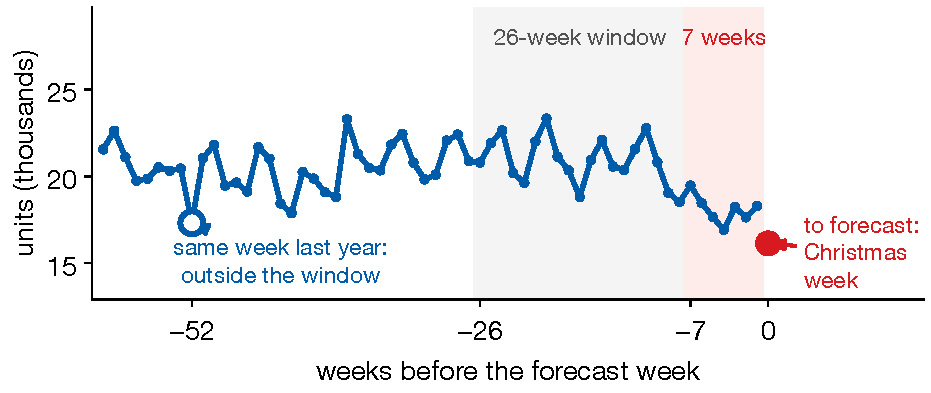
\includegraphics[height=3.9cm]{../Figures/Lecture08/receptive_field.pdf}
  \end{center}
  \vspace{-0.3cm}
  \textbf{The catch is the receptive field.} Stacked width-5 and width-3 filters see seven weeks;
  annual seasonality is 52 away. Add dilation, or feed the annual lag in as its own channel.
\end{frame}

% --- Slide: pipeline ---------------------------------------------------------
\begin{frame}{1D CNN Forecasting Pipeline in PyTorch}
  \begin{examplebox}{Window in, one forecast out}
    {\tiny\linespread{1.2}\selectfont
    \texttt{import torch.nn as nn}\\[2pt]
    \texttt{model = nn.Sequential(}\\
    \texttt{\ \ \ \ nn.Conv1d(n\_channels, 32, kernel\_size=5), nn.ReLU(),}\\
    \texttt{\ \ \ \ nn.Conv1d(32, 64, kernel\_size=3),\ \ \ \ \ \ \ nn.ReLU(),}\\
    \texttt{\ \ \ \ nn.AdaptiveAvgPool1d(1),\ \ \ \# collapses the time axis}\\
    \texttt{\ \ \ \ nn.Flatten(),}\\
    \texttt{\ \ \ \ nn.Linear(64, 1))}
    }
  \end{examplebox}
  Input shape is \texttt{(batch, channels, time)} --- note that channels come \emph{before} time,
  which is the transpose of how the data naturally sits in a dataframe.

  \vspace{0.15cm}
  Everything from Lecture 7 still applies: Adam with weight decay, \texttt{zero\_grad()} every
  batch, \texttt{shuffle=False}, and a split by time rather than at random.

  \vspace{0.1cm}
  \muted{\footnotesize\itshape \texttt{AdaptiveAvgPool1d(1)} averages across the whole time axis.
  Watch what that does on the next slide.}
\end{frame}

% --- Slide: does it work -----------------------------------------------------
\begin{frame}{Does It Actually Work?}
  Fitted on our weekly panel --- 26-week windows, four channels, 30 store-category series, the
  same test block as Homework 4.
  \begin{center}
    {\small
    \begin{tabular}{lrr}
      \toprule
      \textbf{Model} & \textbf{Test RMSE} & \textbf{Parameters} \\
      \midrule
      LASSO (Homework 4) & \textbf{744} & 46 \\
      XGBoost (Homework 4) & 781 & --- \\
      Random forest (Homework 3) & 899 & --- \\
      \midrule
      1D CNN, flatten head & 1{,}032 & 8{,}161 \\
      1D CNN, global max pool & 1{,}418 & 6{,}945 \\
      1D CNN, global average pool & 1{,}534 & 6{,}945 \\
      \midrule
      Seasonal naive & 2{,}152 & 0 \\
      \bottomrule
    \end{tabular}
    }
  \end{center}

  \vspace{-0.2cm}
  \textbf{Every CNN variant loses to a 46-coefficient linear model} --- a seven-week receptive
  field cannot see the annual lag LASSO was handed directly.

  \vspace{0.05cm}
  And swapping average pooling for \texttt{Flatten}, which keeps \emph{where} each pattern
  occurred, is worth about \textbf{500 RMSE} --- three seeds each, against a spread of about 80.
\end{frame}

% =============================================================================
\section{Key Takeaways}
% =============================================================================

\sectionslide{Key Takeaways}{%
  What convolution is for, and what it is not for.}

% --- Slide: architecture summary ---------------------------------------------
\begin{frame}{CNN Architecture Summary}
  \begin{center}
    {\small
    \begin{tabular}{llp{6.6cm}}
      \toprule
      \textbf{Architecture} & \textbf{Year} & \textbf{The idea that survived} \\
      \midrule
      LeNet-5 & 1998 & Conv--pool--conv--pool--dense: the template \\
      VGG & 2014 & Only $3\times3$ filters, stacked deep \\
      Inception & 2014 & Parallel filter sizes; $1\times1$ to cut channels \\
      ResNet & 2015 & Skip connections make real depth trainable \\
      1D CNN & --- & The same machinery along a time axis \\
      \bottomrule
    \end{tabular}
    }
  \end{center}

  \vspace{0.15cm}
  \textbf{Reach for a 1D CNN} when local shape matters more than exact position, when you have
  many parallel series, or as a cheap feature extractor feeding something else.

  \vspace{0.1cm}
  \textbf{Do not reach for one} when the dominant signal is at a long lag, when you have well
  engineered tabular features already, or when a stakeholder needs to read the model. On the
  evidence above, that covers most of what we forecast in this course.
\end{frame}

% --- Slide: Key takeaways ----------------------------------------------------
\begin{frame}{Lecture 8: Key Takeaways}
  \begin{keybox}
    {\small
    \begin{enumerate}\itemsep3pt
      \item \textbf{Convolution} = local connectivity + weight sharing: learn a pattern once,
            find it everywhere.
      \item \textbf{Pooling} buys translation invariance --- which images want and forecasts
            usually don't. Cost here: about 500 RMSE.
      \item Three ideas outlived the architectures: \textbf{small filters stacked deep},
            \textbf{skip connections}, \textbf{learned features}.
      \item A \textbf{1D CNN}'s limit is its \textbf{receptive field}: seven weeks cannot
            see an annual lag.
      \item Every CNN variant \textbf{lost to a 46-coefficient LASSO}. Fit the architecture to
            the problem.
    \end{enumerate}
    }
  \end{keybox}
  \muted{\itshape Next: RNNs and LSTMs --- built to carry state through time.}
\end{frame}

% --- References ---------------------------------------------------------------
\begin{frame}[allowframebreaks]{References}
  \printbibliography[heading=none]
\end{frame}

% =============================================================================
\end{document}
% =============================================================================
